\documentclass[twoside]{book}

% Packages required by doxygen
\usepackage{fixltx2e}
\usepackage{calc}
\usepackage{doxygen}
\usepackage[export]{adjustbox} % also loads graphicx
\usepackage{graphicx}
\usepackage[utf8]{inputenc}
\usepackage{makeidx}
\usepackage{multicol}
\usepackage{multirow}
\PassOptionsToPackage{warn}{textcomp}
\usepackage{textcomp}
\usepackage[nointegrals]{wasysym}
\usepackage[table]{xcolor}

% Font selection
\usepackage[T1]{fontenc}
\usepackage[scaled=.90]{helvet}
\usepackage{courier}
\usepackage{amssymb}
\usepackage{sectsty}
\renewcommand{\familydefault}{\sfdefault}
\allsectionsfont{%
  \fontseries{bc}\selectfont%
  \color{darkgray}%
}
\renewcommand{\DoxyLabelFont}{%
  \fontseries{bc}\selectfont%
  \color{darkgray}%
}
\newcommand{\+}{\discretionary{\mbox{\scriptsize$\hookleftarrow$}}{}{}}

% Page & text layout
\usepackage{geometry}
\geometry{%
  a4paper,%
  top=2.5cm,%
  bottom=2.5cm,%
  left=2.5cm,%
  right=2.5cm%
}
\tolerance=750
\hfuzz=15pt
\hbadness=750
\setlength{\emergencystretch}{15pt}
\setlength{\parindent}{0cm}
\setlength{\parskip}{3ex plus 2ex minus 2ex}
\makeatletter
\renewcommand{\paragraph}{%
  \@startsection{paragraph}{4}{0ex}{-1.0ex}{1.0ex}{%
    \normalfont\normalsize\bfseries\SS@parafont%
  }%
}
\renewcommand{\subparagraph}{%
  \@startsection{subparagraph}{5}{0ex}{-1.0ex}{1.0ex}{%
    \normalfont\normalsize\bfseries\SS@subparafont%
  }%
}
\makeatother

% Headers & footers
\usepackage{fancyhdr}
\pagestyle{fancyplain}
\fancyhead[LE]{\fancyplain{}{\bfseries\thepage}}
\fancyhead[CE]{\fancyplain{}{}}
\fancyhead[RE]{\fancyplain{}{\bfseries\leftmark}}
\fancyhead[LO]{\fancyplain{}{\bfseries\rightmark}}
\fancyhead[CO]{\fancyplain{}{}}
\fancyhead[RO]{\fancyplain{}{\bfseries\thepage}}
\fancyfoot[LE]{\fancyplain{}{}}
\fancyfoot[CE]{\fancyplain{}{}}
\fancyfoot[RE]{\fancyplain{}{\bfseries\scriptsize Generated by Doxygen }}
\fancyfoot[LO]{\fancyplain{}{\bfseries\scriptsize Generated by Doxygen }}
\fancyfoot[CO]{\fancyplain{}{}}
\fancyfoot[RO]{\fancyplain{}{}}
\renewcommand{\footrulewidth}{0.4pt}
\renewcommand{\chaptermark}[1]{%
  \markboth{#1}{}%
}
\renewcommand{\sectionmark}[1]{%
  \markright{\thesection\ #1}%
}

% Indices & bibliography
\usepackage{natbib}
\usepackage[titles]{tocloft}
\setcounter{tocdepth}{3}
\setcounter{secnumdepth}{5}
\makeindex

% Hyperlinks (required, but should be loaded last)
\usepackage{ifpdf}
\ifpdf
  \usepackage[pdftex,pagebackref=true]{hyperref}
\else
  \usepackage[ps2pdf,pagebackref=true]{hyperref}
\fi
\hypersetup{%
  colorlinks=true,%
  linkcolor=blue,%
  citecolor=blue,%
  unicode%
}

% Custom commands
\newcommand{\clearemptydoublepage}{%
  \newpage{\pagestyle{empty}\cleardoublepage}%
}

\usepackage{caption}
\captionsetup{labelsep=space,justification=centering,font={bf},singlelinecheck=off,skip=4pt,position=top}

%===== C O N T E N T S =====

\begin{document}

% Titlepage & ToC
\hypersetup{pageanchor=false,
             bookmarksnumbered=true,
             pdfencoding=unicode
            }
\pagenumbering{alph}
\begin{titlepage}
\vspace*{7cm}
\begin{center}%
{\Large My Project \\[1ex]\large 1 }\\
\vspace*{1cm}
{\large Generated by Doxygen 1.8.13}\\
\end{center}
\end{titlepage}
\clearemptydoublepage
\pagenumbering{roman}
\tableofcontents
\clearemptydoublepage
\pagenumbering{arabic}
\hypersetup{pageanchor=true}

%--- Begin generated contents ---
\chapter{File Index}
\section{File List}
Here is a list of all files with brief descriptions\+:\begin{DoxyCompactList}
\item\contentsline{section}{/home/kavya/\+Desktop/csn261\+\_\+lab\+\_\+assignment1/q1/code/\hyperlink{q1_8c}{q1.\+c} }{\pageref{q1_8c}}{}
\end{DoxyCompactList}

\chapter{File Documentation}
\hypertarget{q2_8c}{}\section{/home/kavya/\+Desktop/ass3/q2/code/q2.c File Reference}
\label{q2_8c}\index{/home/kavya/\+Desktop/ass3/q2/code/q2.\+c@{/home/kavya/\+Desktop/ass3/q2/code/q2.\+c}}
{\ttfamily \#include $<$stdio.\+h$>$}\newline
{\ttfamily \#include $<$stdlib.\+h$>$}\newline
{\ttfamily \#include $<$string.\+h$>$}\newline
{\ttfamily \#include $<$time.\+h$>$}\newline
Include dependency graph for q2.\+c\+:\nopagebreak
\begin{figure}[H]
\begin{center}
\leavevmode
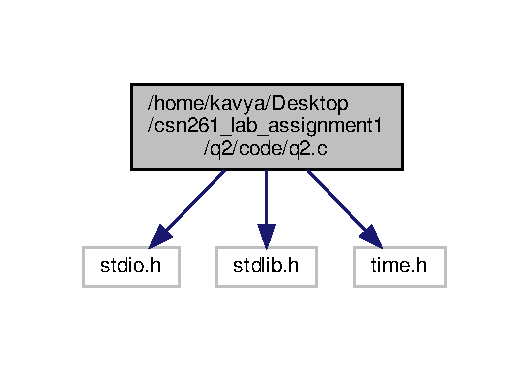
\includegraphics[width=322pt]{q2_8c__incl}
\end{center}
\end{figure}
\subsection*{Data Structures}
\begin{DoxyCompactItemize}
\item 
struct \hyperlink{struct_q_node}{Q\+Node}
\item 
struct \hyperlink{struct_node}{Node}
\end{DoxyCompactItemize}
\subsection*{Functions}
\begin{DoxyCompactItemize}
\item 
void \hyperlink{q2_8c_a7a66c9c39737ce2ae76c39b76c525ef5}{store} (int ii, int jj, int kk)
\item 
void \hyperlink{q2_8c_a55c3cc33aa878501ddb38eda82bbcbe8}{insert} (int d)
\item 
int $\ast$$\ast$ \hyperlink{q2_8c_a04ca5bc036521effb2e480ce1dd434d3}{X\+O\+Ri2l} (int l)
\item 
int \hyperlink{q2_8c_a1bfecc4b0eeeb0004c1053d4a035f65b}{count} (int $\ast$$\ast$X\+OR, int i, int k, int l)
\item 
int \hyperlink{q2_8c_aee2d51a67941e729b1ac66436a674e9c}{count\+Triplets} (int l)
\item 
void \hyperlink{q2_8c_a4b05ced400ef492052a1d50e2755d71a}{show\+Triplets} ()
\item 
int \hyperlink{q2_8c_ae66f6b31b5ad750f1fe042a706a4e3d4}{main} ()
\end{DoxyCompactItemize}
\subsection*{Variables}
\begin{DoxyCompactItemize}
\item 
struct \hyperlink{struct_q_node}{Q\+Node} $\ast$ \hyperlink{q2_8c_a8de334d1886e53de23eaa398ef719c10}{Qfirst} = N\+U\+LL
\item 
struct \hyperlink{struct_q_node}{Q\+Node} $\ast$ \hyperlink{q2_8c_a8ca821529cf5c5bb7f4e55c8d756b64f}{Qlast} =N\+U\+LL
\item 
struct \hyperlink{struct_node}{Node} $\ast$ \hyperlink{q2_8c_ad4f551b04c42cff59f7823e0ec1bc90e}{first} = N\+U\+LL
\item 
struct \hyperlink{struct_node}{Node} $\ast$ \hyperlink{q2_8c_ad55f91e3773370b790704d512696ad6d}{last} =N\+U\+LL
\item 
int \hyperlink{q2_8c_a9f59b34b1f25fe00023291b678246bcc}{length} =0
\end{DoxyCompactItemize}


\subsection{Function Documentation}
\mbox{\Hypertarget{q2_8c_a1bfecc4b0eeeb0004c1053d4a035f65b}\label{q2_8c_a1bfecc4b0eeeb0004c1053d4a035f65b}} 
\index{q2.\+c@{q2.\+c}!count@{count}}
\index{count@{count}!q2.\+c@{q2.\+c}}
\subsubsection{\texorpdfstring{count()}{count()}}
{\footnotesize\ttfamily int count (\begin{DoxyParamCaption}\item[{int $\ast$$\ast$}]{X\+OR,  }\item[{int}]{i,  }\item[{int}]{k,  }\item[{int}]{l }\end{DoxyParamCaption})}

Helper method for count\+Triplets ,which counts triplets using the 2-\/d array X\+O\+R(lookup table) 
\begin{DoxyParams}{Parameters}
{\em X\+OR} & 2-\/d integer array , whose i,j entry denotes the X\+OR of ith input to jth input. \\
\hline
{\em i} & integer i for (i , j , k) \\
\hline
{\em k} & integer i for (i , j , k) \\
\hline
{\em l} & integer length , of the given linked list. \\
\hline
\end{DoxyParams}
\begin{DoxyAuthor}{Author}
Kavya Barnwal 
\end{DoxyAuthor}
\begin{DoxyDate}{Date}
20/08/2019 
\end{DoxyDate}


Definition at line 109 of file q2.\+c.

\mbox{\Hypertarget{q2_8c_aee2d51a67941e729b1ac66436a674e9c}\label{q2_8c_aee2d51a67941e729b1ac66436a674e9c}} 
\index{q2.\+c@{q2.\+c}!count\+Triplets@{count\+Triplets}}
\index{count\+Triplets@{count\+Triplets}!q2.\+c@{q2.\+c}}
\subsubsection{\texorpdfstring{count\+Triplets()}{countTriplets()}}
{\footnotesize\ttfamily int count\+Triplets (\begin{DoxyParamCaption}\item[{int}]{l }\end{DoxyParamCaption})}

This method will be used to count all the possibles triplets i ,j ,k . 
\begin{DoxyParams}{Parameters}
{\em l} & integer length , of the given linked list. \\
\hline
\end{DoxyParams}
\begin{DoxyAuthor}{Author}
Kavya Barnwal 
\end{DoxyAuthor}
\begin{DoxyDate}{Date}
20/08/2019 
\end{DoxyDate}


Definition at line 126 of file q2.\+c.

\mbox{\Hypertarget{q2_8c_a55c3cc33aa878501ddb38eda82bbcbe8}\label{q2_8c_a55c3cc33aa878501ddb38eda82bbcbe8}} 
\index{q2.\+c@{q2.\+c}!insert@{insert}}
\index{insert@{insert}!q2.\+c@{q2.\+c}}
\subsubsection{\texorpdfstring{insert()}{insert()}}
{\footnotesize\ttfamily void insert (\begin{DoxyParamCaption}\item[{int}]{d }\end{DoxyParamCaption})}

This method will be used to store the the given value d into a new node which will bw inserted in the linked list. 
\begin{DoxyParams}{Parameters}
{\em d} & integer data provided to insert in the linked list. \\
\hline
\end{DoxyParams}
\begin{DoxyAuthor}{Author}
Kavya Barnwal 
\end{DoxyAuthor}
\begin{DoxyDate}{Date}
20/08/2019 
\end{DoxyDate}


Definition at line 50 of file q2.\+c.

\mbox{\Hypertarget{q2_8c_ae66f6b31b5ad750f1fe042a706a4e3d4}\label{q2_8c_ae66f6b31b5ad750f1fe042a706a4e3d4}} 
\index{q2.\+c@{q2.\+c}!main@{main}}
\index{main@{main}!q2.\+c@{q2.\+c}}
\subsubsection{\texorpdfstring{main()}{main()}}
{\footnotesize\ttfamily int main (\begin{DoxyParamCaption}{ }\end{DoxyParamCaption})}

initializing the clock 

Definition at line 153 of file q2.\+c.

\mbox{\Hypertarget{q2_8c_a4b05ced400ef492052a1d50e2755d71a}\label{q2_8c_a4b05ced400ef492052a1d50e2755d71a}} 
\index{q2.\+c@{q2.\+c}!show\+Triplets@{show\+Triplets}}
\index{show\+Triplets@{show\+Triplets}!q2.\+c@{q2.\+c}}
\subsubsection{\texorpdfstring{show\+Triplets()}{showTriplets()}}
{\footnotesize\ttfamily void show\+Triplets (\begin{DoxyParamCaption}{ }\end{DoxyParamCaption})}

This method will be used to print all the possibles triplets i ,j ,k . \begin{DoxyAuthor}{Author}
Kavya Barnwal 
\end{DoxyAuthor}
\begin{DoxyDate}{Date}
20/08/2019 
\end{DoxyDate}


Definition at line 145 of file q2.\+c.

\mbox{\Hypertarget{q2_8c_a7a66c9c39737ce2ae76c39b76c525ef5}\label{q2_8c_a7a66c9c39737ce2ae76c39b76c525ef5}} 
\index{q2.\+c@{q2.\+c}!store@{store}}
\index{store@{store}!q2.\+c@{q2.\+c}}
\subsubsection{\texorpdfstring{store()}{store()}}
{\footnotesize\ttfamily void store (\begin{DoxyParamCaption}\item[{int}]{ii,  }\item[{int}]{jj,  }\item[{int}]{kk }\end{DoxyParamCaption})}

This method will be used to store the i ,j ,k values in the linked list. 
\begin{DoxyParams}{Parameters}
{\em ii} & integer i for (i , j , k) \\
\hline
{\em jj} & integer i for (i , j , k) \\
\hline
{\em kk} & integer i for (i , j , k) \\
\hline
\end{DoxyParams}
\begin{DoxyAuthor}{Author}
Kavya Barnwal 
\end{DoxyAuthor}
\begin{DoxyDate}{Date}
20/08/2019 
\end{DoxyDate}


Definition at line 20 of file q2.\+c.

\mbox{\Hypertarget{q2_8c_a04ca5bc036521effb2e480ce1dd434d3}\label{q2_8c_a04ca5bc036521effb2e480ce1dd434d3}} 
\index{q2.\+c@{q2.\+c}!X\+O\+Ri2l@{X\+O\+Ri2l}}
\index{X\+O\+Ri2l@{X\+O\+Ri2l}!q2.\+c@{q2.\+c}}
\subsubsection{\texorpdfstring{X\+O\+Ri2l()}{XORi2l()}}
{\footnotesize\ttfamily int$\ast$$\ast$ X\+O\+Ri2l (\begin{DoxyParamCaption}\item[{int}]{l }\end{DoxyParamCaption})}

This method generates a lookup table for X\+OR outputs from ith entry of linked list to jth entry ,and stores and return a 2-\/d array whose i,j entry denotes the X\+OR of ith input to jth input. 
\begin{DoxyParams}{Parameters}
{\em l} & integer length , of the given linked list. \\
\hline
\end{DoxyParams}
\begin{DoxyAuthor}{Author}
Kavya Barnwal 
\end{DoxyAuthor}
\begin{DoxyDate}{Date}
20/08/2019 
\end{DoxyDate}


Definition at line 74 of file q2.\+c.



\subsection{Variable Documentation}
\mbox{\Hypertarget{q2_8c_ad4f551b04c42cff59f7823e0ec1bc90e}\label{q2_8c_ad4f551b04c42cff59f7823e0ec1bc90e}} 
\index{q2.\+c@{q2.\+c}!first@{first}}
\index{first@{first}!q2.\+c@{q2.\+c}}
\subsubsection{\texorpdfstring{first}{first}}
{\footnotesize\ttfamily struct \hyperlink{struct_node}{Node}$\ast$ first = N\+U\+LL}



Definition at line 41 of file q2.\+c.

\mbox{\Hypertarget{q2_8c_ad55f91e3773370b790704d512696ad6d}\label{q2_8c_ad55f91e3773370b790704d512696ad6d}} 
\index{q2.\+c@{q2.\+c}!last@{last}}
\index{last@{last}!q2.\+c@{q2.\+c}}
\subsubsection{\texorpdfstring{last}{last}}
{\footnotesize\ttfamily struct \hyperlink{struct_node}{Node} $\ast$ last =N\+U\+LL}



Definition at line 41 of file q2.\+c.

\mbox{\Hypertarget{q2_8c_a9f59b34b1f25fe00023291b678246bcc}\label{q2_8c_a9f59b34b1f25fe00023291b678246bcc}} 
\index{q2.\+c@{q2.\+c}!length@{length}}
\index{length@{length}!q2.\+c@{q2.\+c}}
\subsubsection{\texorpdfstring{length}{length}}
{\footnotesize\ttfamily int length =0}



Definition at line 42 of file q2.\+c.

\mbox{\Hypertarget{q2_8c_a8de334d1886e53de23eaa398ef719c10}\label{q2_8c_a8de334d1886e53de23eaa398ef719c10}} 
\index{q2.\+c@{q2.\+c}!Qfirst@{Qfirst}}
\index{Qfirst@{Qfirst}!q2.\+c@{q2.\+c}}
\subsubsection{\texorpdfstring{Qfirst}{Qfirst}}
{\footnotesize\ttfamily struct \hyperlink{struct_q_node}{Q\+Node}$\ast$ Qfirst = N\+U\+LL}



Definition at line 10 of file q2.\+c.

\mbox{\Hypertarget{q2_8c_a8ca821529cf5c5bb7f4e55c8d756b64f}\label{q2_8c_a8ca821529cf5c5bb7f4e55c8d756b64f}} 
\index{q2.\+c@{q2.\+c}!Qlast@{Qlast}}
\index{Qlast@{Qlast}!q2.\+c@{q2.\+c}}
\subsubsection{\texorpdfstring{Qlast}{Qlast}}
{\footnotesize\ttfamily struct \hyperlink{struct_q_node}{Q\+Node} $\ast$ Qlast =N\+U\+LL}



Definition at line 10 of file q2.\+c.


%--- End generated contents ---

% Index
\backmatter
\newpage
\phantomsection
\clearemptydoublepage
\addcontentsline{toc}{chapter}{Index}
\printindex

\end{document}
